% CHAPTER 5

\setcounter{chapter}{4}
\chapter{The Vocal Tract and Linear Predictive Coding}
\thispagestyle{plain}

%Box with Learning objectives should be at the beginning of each chapter
\begin{corollary}

	\hspace*{10mm}
	
	\vspace{5mm} %for optical corrections
	% optionaler Text	
	
	\begin{itemize}
			\item Tube Model of the Vocal Tract
			\item Linear Prediction
			
	\end{itemize}
\end{corollary}

\newpage

% CHAPTER 5 LESSON 1

\section{Tube Model of the Vocal Tract}
\label{Tube Model of the Vocal Tract}


The first chapter introduced the concept of the source filter model for speech production. In this model an excitiation source (air pushed from the lungs) is passed through a filter (the vocal tract) to produce speech. Air pushed from the lungs can be periodically regulated by the glottus producing a voiced speech sound.  When the glottus is not used, and air is simply pushed through the vocal tract, an unvoiced sound is produced. Because the vocal tract is not perfectly cylindrical, reflections occur. These reflections produce resonances, also called formants, that are critical for distinguishing speech sounds. 

\begin{figure}[h]
	\centering
	 \def\svgwidth{10cm}
	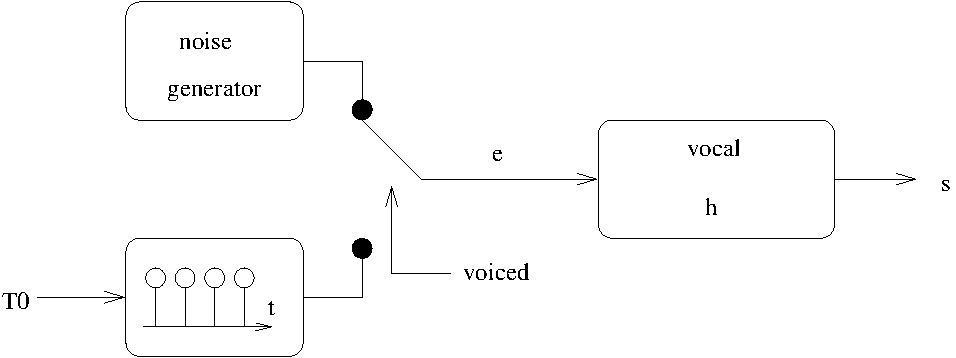
\includegraphics[width=0.5\linewidth]{Pictures/Chapter3_Lesson3/filterVUv2-eps-converted-to.pdf}
	\caption{Source filter model of the vocal tract}
	\label{fig:SourceFil}
\end{figure}

Figure 3.1 displays the method that will be sued to model the excitation sources. Voiced speech is modelled as a pulse train, whereas random noise is used to model unvoiced speech.  Note that there is a switch in the diagram implying that the model will require some sort of detection to switch between the two sources. 

Now we want a model for speech production.  We therefore decompose speech into excitation souorce and spectral shape. The excitation source can be modelled as a pulse train. Unvoiced can be a random noise generator.  Also can be used for mixed excitiation. 

The second part is the vocal tract filter that can be modelled by a tube where we ignore the nasal tract because it is complicated.

What we want is a mathematical model for the vocal tract. Once we have this model, then we can estimate the parameters that describe the shape of our voacl tract only from the speech recording. We start with what is phsically going on in the vocal tract.

We know that sound is a pressure wave.  That there air particles in it that oscillate back and forth.  There are area of compression and areas of refraction.  

WE now consider a pressure wave within a tube.  The interaction of the particles with the tube ends whteher open or closed introduces boundary conditions to the problem, that affect the propagation of the wave through the medium.  At the open end the pressure wave is forced to have a minimum, at the closed end, it is forced to have a maximum.

We define pressure P(x,t), v(x,t) V(x,t) from these, we can define an acoustical impedance.

Whenever there is a change in impedance, we have a reflection.  This can be charaterized by a reflection coefficient that is a function of the acoustical impedance of the two media.

Put in equations

The close end = pressure maximum, velocity minimum (particles cant move.)
open end = opposite

put into equations we see that

 at the closed end, the reflection coefficient goes to -1

at the open end, we have a reflection with +1

This now implies that we have a backward travelling wave from the open end reflection.  The forward wave and the backward wave will add up. They will add up if they match the resonance frequency of the tube. 

picture of tube with wavelengths.  Derivation of equations for vocal tract resonances. One resonance per kHz!!!! Approx 4 resonances per kHz. However if this was the case with our vocal tract, speech would be unintelligible because the formants do not change.  Becasue we cannot alter the length of our vocal tract, we can instead constrict certian parts to change the postion of the resonances. We have to therefore model the voacl tract as a tube with individual segments that change their shpae over time.

pictiure

We can treat this as a set of short indivudal tubes and do the same computations for each segment as we did for the tube.  We can then concatenate the results to get our filter.

SO we have short cylindrical tubes with different areas 

equations

Assumptions:
low friction, plane wave prop

Therefore we can use equations for pressure and volum velocity 


% CHAPTER 5 LESSON 2

\newcommand{\indexTime}{n}
\newcommand{\convIndex}{m}
\newcommand{\excitationFunc}{e}
\newcommand{\filterFunc}{h}
\newcommand{\filtOutFunc}{s}
\newcommand{\predictionError}{d}
\newcommand{\Error}{E}
\newcommand{\newIndex}{\mu}
\newcommand{\autoCorr}{\phi_{s}}
\newcommand{\maConvIndex}{m}
\newcommand{\arConvIndex}{\nu}
\newcommand{\maFiltOrder}{q}
\newcommand{\arFiltOrder}{p}
\newcommand{\maFiltCoef}{b}
\newcommand{\arFiltCoef}{a}


\section{Linear Prediction}
\label{Linear Prediction}


\begin{itemize}

\item Goal: Find a model for the vocal tract filter from a speech signal.

\item In general, this filter can be modelled as infintitely long

\begin{equation}\filtOutFunc(\indexTime) = \sum^{\infty}_{\convIndex = 0} \filterFunc(\convIndex)\excitationFunc(\indexTime-\convIndex)\end{equation}

\item The infinite sum can be replaced by a finite recursive equation.
ARMA model 

\begin{equation}\filtOutFunc(\indexTime) = \sum^{\maFiltOrder}_{\maConvIndex = 0}\maFiltCoef_{\maConvIndex }\excitationFunc(\indexTime-\maConvIndex) -  \sum^{\arFiltOrder}_{\arConvIndex = 1}\arFiltCoef_{\arConvIndex }\filtOutFunc(\indexTime-\arConvIndex)\end{equation}

\begin{equation}\MakeUppercase{\filtOutFunc}(z) =\MakeUppercase{\excitationFunc}(z) \sum^{\maFiltOrder}_{\maConvIndex = 0}\maFiltCoef_{\maConvIndex }z^{-\maConvIndex} -  \MakeUppercase{\filtOutFunc}(z) \sum^{\arFiltOrder}_{\arConvIndex = 1}\arFiltCoef_{\arConvIndex }z^{-\arConvIndex}\end{equation}

\begin{equation}\MakeUppercase{\filtOutFunc}(z)(1 +  \sum^{\arFiltOrder}_{\arConvIndex = 1}\arFiltCoef_{\arConvIndex }z^{-\arConvIndex}) =\MakeUppercase{\excitationFunc}(z) \sum^{\maFiltOrder}_{\maConvIndex = 0}\maFiltCoef_{\maConvIndex }z^{-\maConvIndex} \end{equation}

\item In the Z domain, we can define the transfer function 
\begin{equation}\MakeUppercase{\filterFunc}(z)  = \frac{\MakeUppercase{\filtOutFunc}(z)}{\MakeUppercase{\excitationFunc}(z)} = \frac{ \sum\limits^{\maFiltOrder}_{\maConvIndex = 0}\maFiltCoef_{\maConvIndex }z^{-\maConvIndex}}{\sum\limits^{\arFiltOrder}_{\arConvIndex = 0}\arFiltCoef_{\arConvIndex }z^{-\arConvIndex}}     |_{a_0 = 1}\end{equation}



\begin{itemize}
\item Transfer function consists of two polynomials-

\item Fundamental theorem of algebra

\begin{itemize}

\item  ''Every non-zero single variable polynomial has at least one root.''  polynomial of order n has n roots

\item A polynomial in z can be divided by (z-a)

\begin{itemize}

\item \begin{equation*}  \frac{p(z)}{(z-a)} = q(z) + \frac{R}{z-a}\mbox{\begin{math}\implies\end{math} R: not a function of z}\end{equation*}

\item \begin{equation*}p(z) = (z-a)q(z) + R\mbox{\begin{math}\implies\end{math}q(z) is a polynmomial w than p(z)}\end{equation*}

\item if \begin{math} a = z_0\end{math} is a root, then
\begin{equation*}p(z_0) = 0 =  (z_0-z_0)q(z) + R\mbox{ \begin{math}\implies\end{math}  R = 0}\end{equation*}

\item  if \begin{math} a = z_0 \implies\end{math} is a root, then the residual is zero

\end{itemize}
\item \begin{math}\implies\end{math}  Every polynomial can be factorized by its roots
\end{itemize}
\end{itemize}


\item \begin{equation*}\MakeUppercase{\filterFunc}(z)  = \frac{\MakeUppercase{\filtOutFunc}(z)}{\MakeUppercase{\excitationFunc}(z)} = \frac{\sum\limits^{\maFiltOrder}_{\maConvIndex = 0}\maFiltCoef_{\maConvIndex }z^{-\maConvIndex}}{\sum\limits^{\arFiltOrder}_{\arConvIndex = 0}\arFiltCoef_{\arConvIndex }z^{-\arConvIndex}}     |_{a_0 = 1} =\frac{\maFiltCoef_0z^{-\maFiltOrder}}{z^{-\arFiltOrder}}\frac{z^{\maFiltOrder}+\frac{\maFiltCoef_1}{\maFiltCoef_0}z^{\maFiltOrder-1}+...+\frac{\maFiltCoef_{\maFiltOrder}}{\maFiltCoef_0}}{z^{\arFiltOrder}+\arFiltCoef_1z^{\arFiltOrder-1}+...+\arFiltCoef_{\arFiltOrder}} = b_0\frac{z^{-\maFiltOrder}}{z^{-\maFiltOrder}}\frac{\prod\limits^{\maFiltOrder}_{\maConvIndex=1}(z - z_{0_{\maConvIndex}})}{\prod\limits^{\arFiltOrder}_{\arConvIndex = 1}(z - z_{0_{\arConvIndex}})}\end{equation*}

\begin{equation*}\mbox{\begin{math}z_{0_{\maConvIndex}}\end{math}: Roots of numerator polynomial  \begin{math}\implies\end{math} zeros of \MakeUppercase{\filterFunc}(z)}\end{equation*}

\begin{equation*}\mbox{\begin{math}z_{0_{\arConvIndex}}\end{math}: Roots of denominator polynomial  \begin{math}\implies\end{math} poles of \MakeUppercase{\filterFunc}(z)}\end{equation*}

\item{pole/zero model (Z-domain) \begin{math}\rightleftharpoons\end{math}ARMA model (time-domain) }

\begin{itemize}

\item MA process / all zero filter

\begin{equation}\filtOutFunc(\indexTime) = \sum_{\maConvIndex = 1}^{\maFiltOrder}\maFiltCoef_{\maConvIndex}\excitationFunc(\indexTime - \maConvIndex)\mbox{ \begin{math}\rightarrow\end{math}time domain}\end{equation}

\begin{equation}\MakeUppercase{\filtOutFunc}(z) = \MakeUppercase{\excitationFunc}(z)z^{-\maFiltOrder}\maFiltCoef_0 \prod\limits^{\maFiltOrder}_{\maConvIndex=1}(z - z_{0_{\maConvIndex}})\mbox{\begin{math}\rightarrow\end{math}frequency- domain}\end{equation}

\item AR process/all pole filter

\begin{equation}\filtOutFunc(\indexTime) = \maFiltCoef_0\excitationFunc(\indexTime) - \sum_{\arConvIndex =  1}^{\arFiltOrder}\arFiltCoef_{\arConvIndex}\filtOutFunc(\indexTime - \arConvIndex)\mbox{ \begin{math}\rightarrow\end{math}time domain}\end{equation}

\begin{equation}\MakeUppercase{\filtOutFunc}(z) = \MakeUppercase{\excitationFunc}(z)\maFiltCoef_0 \frac{z^{\arFiltOrder}}{\prod\limits^{\arFiltOrder}_{\arConvIndex=1}(z-z_{0_{\arConvIndex}})}\mbox{\begin{math}\rightarrow\end{math}frequency- domain}\end{equation}

\end{itemize}

\item This recursive structure resembles the recursive structure obtained from the tube model. (Nasal tract, glottal and labial filter neglected)

\begin{itemize}

\item The amplitude characteristics can be apporximated by increasing AR filter order

\item We are less sensitive to phase as compared to amplitude changes

\end{itemize}

\item Advantages of the AR Model

\begin{itemize}

\item Always invertible if stable

\item Coefficients can be efficiently obtained

\end{itemize}

\end{itemize}


\subsection{Computation of AR coefficients}

AR Model
\begin{equation}\filtOutFunc(\indexTime) = \maFiltCoef_0\excitationFunc(\indexTime) - \sum_{\arConvIndex =  1}^{\arFiltOrder}\arFiltCoef_{\arConvIndex}\filtOutFunc(\indexTime - \arConvIndex)\end{equation}

\begin{itemize}

\item Successive speech samples are correlated

\item at time n, \filtOutFunc(\indexTime) can be predicted up to the innovation, \begin{math}\maFiltCoef_0\excitationFunc(\indexTime)\end{math}.

\begin{equation*}\mbox{Prediction: }\hat{\filtOutFunc}(\indexTime) = - \sum_{\arConvIndex =  1}^{\arFiltOrder}\hat{\arFiltCoef_{\arConvIndex}}\filtOutFunc(\indexTime - \arConvIndex)\end{equation*}

\begin{equation*}\mbox{for \begin{math}\hat{a_{\arConvIndex}}=a_{\arConvIndex}\end{math} we can predict the speech signal up tot he scaled excitiation}\end{equation*}

\begin{equation*}\predictionError(\indexTime)=\filtOutFunc(\indexTime)-\hat{\filtOutFunc}(\indexTime)=\maFiltCoef_0\excitationFunc(\indexTime)  \end{equation*}

\item find MMSE optimal parameters  \begin{math}\hat{a_{\arConvIndex}}=a_{\arConvIndex}\end{math} by minimizing the mean of the squared error signal

\begin{equation*}\mbox{Approach: Minimize}\MakeUppercase{\excitationFunc}(\predictionError^2)\mbox{How? Set the first derivative to zero}\end{equation*}

\begin{equation*}0 \stackrel{!}{=} \frac{\partial\Error(\predictionError^2(\indexTime)}{\partial\hat{a_{\arConvIndex}}} \stackrel{chain rule}{=}\Error(2\predictionError(\indexTime)\frac{\partial}{\partial\hat{a_{\arConvIndex}}}(\filtOutFunc(\indexTime) + \sum_{\arConvIndex =  1}^{\arFiltOrder}\hat{\arFiltCoef_{\arConvIndex}}\filtOutFunc(\indexTime - \arConvIndex))\end{equation*}

\begin{equation*} = \Error(2\predictionError(\indexTime)\filtOutFunc(\indexTime - \arConvIndex))\end{equation*}


\begin{equation*}=2\Error((\filtOutFunc(\indexTime) + \sum_{\arConvIndex =  1}^{\arFiltOrder}\hat{\arFiltCoef_{\arConvIndex}}\filtOutFunc(\indexTime - \arConvIndex))\filtOutFunc(\indexTime - \arConvIndex))\end{equation*}


\begin{equation*}= \Error(\filtOutFunc(\indexTime)\filtOutFunc(\indexTime - \arConvIndex))+  \sum_{\newIndex =  1}^{\arFiltOrder}\hat{\arFiltCoef_{\newIndex}}\filtOutFunc(\indexTime - \newIndex)\filtOutFunc(\indexTime - \arConvIndex) \end{equation*}

\begin{equation*}\autoCorr(\arConvIndex) =  \Error(\filtOutFunc(\indexTime)\filtOutFunc(\indexTime - \arConvIndex))\end{equation*}


\begin{equation*}=\autoCorr(\arConvIndex) + \sum_{\newIndex =  1}^{\arFiltOrder}\hat{\arFiltCoef_{\newIndex}}\autoCorr(\arConvIndex -\newIndex) \end{equation*}


\begin{equation*}\mbox{Second Derivative}\end{equation*}


\begin{equation*} \frac{\partial^2\Error(\predictionError^2(\indexTime)}{\partial\hat{a_{\arConvIndex}}^2}=\Error(2\autoCorr(0))\geq 0 \rightarrow minimum\end{equation*}

\item Solution to all \begin{math}\hat{a_{\arConvIndex}}\end{math} Wiener Hopf equations/Normal equations. Write in matrix form.

\begin{equation*}\autoCorr(\arConvIndex)=-\sum_{\newIndex =  1}^{\arFiltOrder}\hat{\arFiltCoef_{\newIndex}}\autoCorr(\arConvIndex -\newIndex)=-(\autoCorr(\arConvIndex-1)\hat{a_1} + \autoCorr(\arConvIndex-1)\hat{a_1} + \autoCorr(\arConvIndex-2)\hat{a_2} + \dots +\autoCorr(\arConvIndex-\arFiltOrder)\hat{a_\arFiltOrder} )\end{equation*}

\begin{equation*}\begin{pmatrix}
\autoCorr(1) \\ \autoCorr(2) \\ \vdots \\ \autoCorr(\arFiltOrder)
\end{pmatrix}=-\begin{pmatrix}\autoCorr(0) & \autoCorr(-1) & \autoCorr(-2) & \ldots & \autoCorr(1 -\arFiltOrder) \\
\autoCorr(1) & \autoCorr(0) & \autoCorr(-1) & \ldots & \autoCorr(2 -\arFiltOrder) \\
\vdots & \vdots & \vdots & \ddots & \vdots \\
\autoCorr(\arFiltOrder-1) & \autoCorr(\arFiltOrder-2) & \autoCorr(\arFiltOrder-3) & \ldots & \autoCorr(0)\\ \end{pmatrix}\begin{pmatrix}\hat{\arFiltCoef}_1 \\ \hat{\arFiltCoef}_2 \\ \vdots \\ \hat{\arFiltCoef_{\arFiltOrder}}\end{pmatrix}\end{equation*}

\begin{equation*} \mathbf{\autoCorr} = -\mathbf{R_s}\mathbf{\hat{\arFiltCoef}}\end{equation*}

\begin{equation*} \mbox{Solution to the Wiener Hopf equations gives MMSE-optimal linear predictive coefficients} \hat{\arFiltCoef_\arConvIndex}\end{equation*}

\begin{equation*} \implies \mathbf{\hat{\arFiltCoef}_{opt}}= -\mathbf{R_s}^{-1}\mathbf{\autoCorr} \end{equation*}

\item In Practice: Speech is only short time stationary
\begin{itemize}
\item Estimate autocorrelation on short segements

\item Use temporal averaging instead of E{}
\end{itemize}

\begin{equation*} \mbox{In the so called autocorrelation method,} \mathbf{R_s} \mbox{is estimated on short framed segents } \widetilde{s} \end{equation*}

\begin{equation*}\widetilde{\autoCorr}(\arConvIndex)=\sum^{n_t}_{n = n_1}\widetilde{\filtOutFunc}(\indexTime)\widetilde{\filtOutFunc}(\indexTime - \arConvIndex)\end{equation*}

\item the estimate is symmetric \begin{math}\hat{\autoCorr}(\arConvIndex) = \hat{\autoCorr}(-\arConvIndex)\end{math}

\item the correlation matrix estimate \begin{math}\mathbf{R_s}\end{math} is symmetric and Toeplitz

\item fast solutions (Levinson-Durbin recursion)


\end{itemize}
